\documentclass{article}
\usepackage{graphicx}
\usepackage{subcaption}

\begin{document}
	\begin{figure}[h!]
		\centering
		\begin{subfigure}[b]{0.2\linewidth}
		
		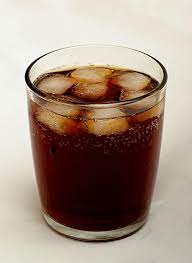
\includegraphics[width=\linewidth]{drink.jpg}
		    \caption{Cola.} \end{subfigure}
	    \begin{subfigure}[b]{0.2\linewidth}
	    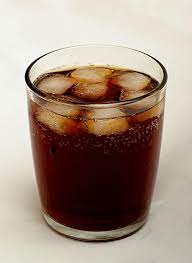
\includegraphics[width=\linewidth]{drink.jpg}
	    \caption{More cola.}
	    \end{subfigure}
         \begin{subfigure}[b]{0.2\linewidth}
        	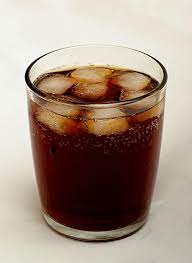
\includegraphics[width=\linewidth]{drink.jpg}
        	\caption{Sweet cola.}
        \end{subfigure}
         \begin{subfigure}[b]{0.5\linewidth}
        	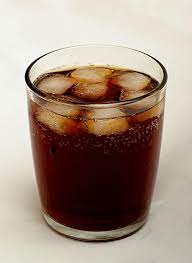
\includegraphics[width=\linewidth]{drink.jpg}
        	\caption{Too much cola.}
        \end{subfigure}
        \caption{The same glass of cola. Multiple times. Want some?}
        \label{fig:cola}
	\end{figure}
\end{document}